\documentclass[11pt,a4paper]{report}
% ---- packages ----
\usepackage{geometry}
 \geometry{
 a4paper,
 total={210mm,297mm},
 left=20mm,
 right=20mm,
 top=30mm,
 bottom=30mm,
 }

\usepackage[utf8]{inputenc}
\usepackage[cyr]{aeguill}
\usepackage{wrapfig}
\usepackage{graphicx}
\usepackage{color}
\usepackage{amsmath}
\usepackage{amsfonts}
\usepackage{amssymb}
\usepackage{pdfpages}
\usepackage[tight]{shorttoc}
\usepackage{hyperref}
\usepackage{verbatim}
\usepackage[english]{babel}
\usepackage{csquotes}
\usepackage{enumerate}
\usepackage{booktabs}
\usepackage{multirow}
\usepackage[inline]{enumitem}
\usepackage[
backend=biber,
style=numeric-comp,
citestyle=numeric-comp,
sorting=ynt
]{biblatex}
\usepackage{listings}


% ---- setup ----
\newcommand{\be }{\begin{itemize}\maketitle}
\newcommand{\en }{\end{itemize}}

\addbibresource{bibliography/bibliography.bib}
\addbibresource{bibliography/github.bib}
\addbibresource{bibliography/online.bib}
\addbibresource{bibliography/papers.bib}
\addbibresource{bibliography/rfcs.bib}
\addbibresource{bibliography/wikipedia.bib}

% section numbering up to subsubsection incl.
\setcounter{secnumdepth}{4} %todo: check for paragraph??

% list in toc up to subsection incl.
\setcounter{tocdepth}{2}

\setlength{\parskip}{1em}

\begin{document}
\renewcommand{\bibname}{References}

% ---- title page ---
\begin{titlepage}

\newcommand{\HRule}{\rule{\linewidth}{0.5mm}}
\center
 
% headings
\textsc{\LARGE Mickaël Misbach Master Thesis}\\[0.5cm]
%\textsc{\LARGE The Hyve}\\[1cm]

\textsc{\Large École Polytechnique Fédérale de Lausanne \& The Hyve}\\[0.5cm] 
\textsc{\large \reportTitle}\\[0.5cm]

% title
\HRule \\[0.4cm]
{ \huge \bfseries Building a common and privacy-preserving front end for open-source clinical research platforms}\\[0.4cm]
%{ \huge \bfseries \reportTitle}\\[0.4cm]
\HRule \\[1cm]
 
% authors
\begin{minipage}{0.4\textwidth}
\begin{flushleft} \large
\emph{Master Student:}\\
Mickaël \textsc{Misbach}$^{*\dagger}$\\
\end{flushleft}
\end{minipage}
~
\begin{minipage}{0.4\textwidth}
\begin{flushright} \large
\emph{The Hyve Supervisors:} \\
Ward \textsc{Weistra}$^*$\\
Dr. Bo \textsc{Gao}$^*$\\[\baselineskip]
\emph{EPFL Supervisors:} \\
Jean-Louis \textsc{Raisaro}$^\dagger$\\
Dr. Juan \textsc{Troncoso-Pastoriza}$^\dagger$\\[\baselineskip]
\emph{EPFL Professor:} \\
Prof. Jean-Pierre \textsc{Hubaux}$^\dagger$\\
\end{flushright}
\end{minipage}\\[1.5cm]


% logos

\includegraphics[width=0.6\linewidth]{./figures/epfl_logo.png}\\

\includegraphics[width=0.66\linewidth]{./figures/thehyve_logo.pdf}\\

% todo: remove the chapter num from the chapte pages?
% todo: tag repo milestone/1, etc. (and place produced bin)
% todo: have internal cover page for all infos (only titles and logos on first)
% todo: use phd template ? https://phd.epfl.ch/page-149270.html
% todo: make look nicer
% todo: add emails as *{firstname}@thehyve.nl ; +{firstname.lastname}@epfl.ch
% todo: The student must write a report that contains the following items:
% The title
% The student’s contact details (surname, first name, address)
% The name of the IC laboratory, the name of the company or the name of the other university in
%which the master thesis is being done
% The name of the responsible IC professor
% The results of the thesis (analysis, conception and implementation)
%The report must be representative of the student’s work in order to be able to judge the student’s ability
%to be an engineer. The project will be archived within the sections and, in general, in the laboratory of the
%IC professor. The report must not contain any confidential information, except in exceptional cases. 

\vfill

\end{titlepage}


% ---- abstract ----
\newpage
\newgeometry{left=3cm,right=3cm}
\begin{abstract}

% problem / motivation
Being able to exploit large and heterogeneous medical data is crucial for realizing the promise of precision medicine to its full potential. 
Yet, currently, due to the presence of multiple and fragmented systems at different clinical sites, it is often difficult to enable researchers to access the data they need. 
Privacy and security concerns also represent major obstacles that need to be overcome in order to provide access to sensitive medical data that are usually not exposed by clinical sites for the fear of data leaks. 

% solution / key idea
To address these challenges, we propose a system that employs Glowing Bear as a common front end to the widespread clinical research platforms i2b2, tranSMART and MedCo.
Our proposed system uses IRCT, the official implementation of the PIC-SURE API, which acts as an interoperability layer that translates clinical research queries into native API languages.
With our work, we take a step towards the technical convergence of i2b2 and tranSMART, giving clinical sites the means to share their data more easily.
Even more, with the support of MedCo, a cohort explorer with strong privacy and security guarantees based on federated i2b2 instances, we enable clinical sites to share sensitive data that would be difficult to share otherwise.

\end{abstract}
\restoregeometry


% --- table of contents pages ----
\newpage
\tableofcontents

% ---- acknowledgements ----
\newpage
\begin{acknowledgements}
TBD
% todo: fam, fri, hyve
\end{acknowledgements}

% ---- content ----
\newpage
\chapter{Introduction}
% a summary of the entire thing
\section{Context/Motivation}


\section{Problem}
-Why this is a hard/open problem?
-State-of-the-Art

\section{Insight}
-Solution overview/some detail (bigger picture)

\section{Summary of research}
-Details of contribution

5 Evidence of successful solution (eg evaluation results)
6 Summary of contributions
7 Paper outline

Intro
Goal: transmart 17.1 - i2b2 - medco (nice to have: shrine, transmart prev. Ver.)
splitted up in 2 obj.
Why open-source

goal: common - privacy preserving

§ the motivation
% todo: get inspiration from papers

§ the goal

These characteristics define two main objectives to fulfill. 
First, the front end in question will need to be able to communicate with the main open-source several clinical research platforms, to cover a major part of the platforms used by researchers.
Second, the front end , namely MedCo, the only privacy-preserving platform.
% todo: in the analyses of what are the platforms, mention what they are

--> focus on cohort exploration

\section{Solution Requirements}
\label{sec:requirements}
- about how we want compatibility with the major open-source clinical research systems
% in CCL: put how the requirements are met 
- use of apis standard to easily integrate with others
- unique front end to exploit several back ends: main open-source ones
- support all the features of GB-> not a requirement, consequence of choosing GB//however a list of the UI features we want to have should be present


todo: define first and second objectives (referenced after)

% todo: ack: hyve ,etc.

% todo: if existing solutions are used: those are used by actual users and should not lose features, no change is desired from user p-o-v

\chapter{Background \& Related Work}
% todo: maybe integrate the sections in the introduction

\section{Background}
% contains purely descriptive information
This section offers some important background information providing context to what is presented in the later chapters. 
First an overview of the different open-source clinical research systems is offered, 
after which the different front ends allowing to exploit them are presented.

\subsection{Clinical Research Systems}

talk about the inner data model of each


\subsubsection{tranSMART}
%TODO

\subsubsection{i2b2}
Informatics for Integrating Biology and the Bedside (i2b2) is a NIH-funded National Center for Biomedical Computing (NCBC) that is developing a software that goes by the same name. 
%todo



%TODO
% core server, demo data
% db compat: 3

\subsubsection{SHRINE}
%TODO

\subsubsection{PIC-SURE API / IRCT}

% overview
The National Institutes of Health (NIH) of the U.S. government launched in 2013 the first phase of the Big Data to Knowledge (BD2K)~\cite{BD2K} whose one of the goal is to exploit the immense amount of big data information to advance knowledge in modern biomedical research.
One of those center of excellence is the PIC-SURE (Patient-centered Information Commons: Standardized Unification of Research Elements)~\cite{PIC-SURE} whose goal is create a scalable toolkit to enable patient-centered information commons.
etc. created within HMS DBMI [cite], open source, 
led by paul avillach One of their achievement is the BD2K PIC-SURE RESTful API [bd2k-picsure.hms.harvard.edu] that aims to incorporate multiple heterogeneous clinical research systems. 
The official implementation of this API is called Inter Resource Communication Tool (IRCT).

% pic-sure api description
While not actually being a clinical research system, the IRCT can be seen as a meta system that expose data of other systems through a common API.
Restful api for heteregeonous datasets ,decentralized fashion, access with single comm. Layer -> interoperability layer (check the api doc pdf)

% IRCT components
The IRCT implementation is the combination of four different components, that are open-source and available on~\cite{IRCT-github}. They are implemented in Java and use standard technologies: web application archive (WAR)~\cite{wiki:war} for deployment, Hibernate~\cite{wiki:hibernate} for data storage.
First the Communication Layer (IRCT-CL) implements the RESTful service that is exposed and documented by~\cite{PIC-SURE-API}. 
The core component is the Application Programming Interface (IRCT-API), it handles the execution of queries and processing of results.
An instance can be extended using the IRCT Extension (IRCT-EXT) that provides hooks and additional features without having to modify the core code.
Finally the Resource Interface (IRCT-RI) connects to the different resources through connectors.


%https://www.nature.com/articles/sdata201696
%http://dbmi.hms.harvard.edu/news/datathon-hackathon-sep-14-15
%info about hackaton: dana farber is looking for i2b2 frontend replacement 

% notes on irct 
%PREDICATE MANDATORY in query
%DATA type is needed in query

\paragraph{Technical Background}
PIC-SURE is resource based: each source of data (e.g. i2b2, tranSMART, etc.) is considered a resource.
Each of these resource declare through their configuration the kind of clauses they support. 
The configuration is done through the database.
Four types of clauses are supported: \emph{select}, \emph{where}, \emph{process} and \emph{join}, but here we are mainly making use of \emph{select} and \emph{where}.

% select
The \emph{select} clauses specify the data that the user of the API wants extracted from the database.
The resources declare what kind of operations their \emph{select} support, for example \emph{AGGREGATE} can be defined to extract aggregated values.
Then each of the operations (or the default operation when none is declared), declare the fields they support.
For \emph{AGGREGATE}, the resource could declare two fields:
\begin{itemize}
    \item \emph{FUNCTION}: what function to use among a list of permitted values, e.g. \emph{COUNT}, \emph{MIN}, \emph{MAX}
    \item \emph{DIMENSION}: the dimension along which to do to the aggregation, e.g. \emph{PATIENT}
\end{itemize}
Each of the fields declare the type of value they take: either an enumerated value, or a data type such as \emph{String} or \emph{Integer} that has to specify the Java class implementing it.
Example of two \emph{select} clauses:
\begin{verbatim}
"select": [ {
    "operation": "AGGREGATE",
    "fields": {
        "FUNCTION": "COUNT",
        "DIMENSION": "PATIENT"
    }
}, {
    "field": {
        "pui": "/resource/study/Age/",
        "dataType": "INTEGER"
    }
} ]
\end{verbatim}

% where 
The other main clause supported is \emph{where} and is used to specified constraints on the data to be selected.
Just like for \emph{select} and the supported operations, the resource declares the predicates that \emph{where} supports.
The predicates can have fields, and fields have a type: this is just like \emph{select}. 
Example:
\begin{verbatim}
"where": [ {
    "field": {
        "pui": ""/resource/study/Age/"",
        "dataType": "INTEGER"
    },
    "predicate": "CONSTRAIN_VALUE_NUMERIC",
    "fields": {
        "OPERATOR": ">=",
        "CONSTRAINT": "20"
    }
} ]
\end{verbatim}

% tree
In order to construct queries made of the clauses previously described, the resources expose a tree of entities.
Each of those entities, if they are queryable, declare a data type.
Each of the predicates used for the \emph{where} clauses also declare one or more supported data types: this is the mechanism used to know which entities support which predicates.

\subsection{Cohort Exploration Front Ends}
\subsubsection{Glowing Bear}
%§ GB: Most recent Angular version is now ng5, AngularJS refers to the first generation of Angular which is sth. glowing bear no longer uses. see https://blog.angular.io/version-5-0-0-of-angular-now-available-37e414935ced

\subsubsection{tranSMARTApp}
%are there other transmart clients that exist?


\subsubsection{i2b2 Clients}
\paragraph{Webclient}

\paragraph{Workbench}

\section{Related Work}
% say if open source or not 
% this is more analytic than background: offering an overview of what else is done and compare it to what we are doing, reuse what was said in the background
%CAVA: http://perer.org/papers/adamPerer-CAVA-IVS2014.pdf

%all the work mentioned in background

%they had a partnership with pic sure: %https://academic.oup.com/jamia/article/22/6/1132/2357622?searchresult=1
%pic sure 'wow' story (nhanes): %https://bd2kccc.org/wp-content/uploads/2017/02/15_PIC-SURE_FInal.pdf

\chapter{System Architecture}
\label{sec:sysarchitecture}

To design a system fulfilling the requirements listed in \ref{sec:requirements}, we start by the bottom with first choosing its basic building blocks, and then we explore the different ways in which they can be assembled.
Following the requirements, we only consider open-source technologies.


\section{Choice of Open-Source Technologies}

% outline
The choice of the open-source technologies to use depends mainly on the clinical research platforms that must be supported, which will be our first step in this section.
We then do a review of the different existing open-source front end systems to determine if one of them is worth being used for our solution.
Finally we motivate the use of an identity provider software and choose one.

\subsection{Back End Systems: Clinical Research Platforms}

% what is a clinical research platform / use-case
A clinical research platform is a back end software (i.e. running on server, serving request to clients), that stores any kind of medical data and can answer queries, with the purpose of identifying patient cohorts, and possibly performing analytics on those data.
Queries on this data can be for any purpose, here follows a few use-cases of this kind of platform.
A medical researcher want to recruit a patient cohort for a study they want to conduct. They need to select patients with a te
pharma testing drugs study
ongologist for persolized medicine: looks for response to treatment of patient according to genes.

% Altogether these systems serve an enormous of data, and being able to access them from a unique front end would prove much beneficial to researchers.

% As stated section~\ref{sec:requirements}, we target compatibility with the main open-source clinical research platforms. 
% In that area the two main players are \emph{i2b2} and \emph{tranSMART}.
% Less widespread, and building on \emph{i2b2}, also exists \emph{SHRINE} and \emph{MedCo}.

% § about i2b2: why support it

% § about tranSMART: why support it 

% § about MedCo: why support it


% what exist there, which one we are targetting the compatibility for and why // descriptive part in related work / background



\begin{itemize}
    \item why using IRCT and not i2b2 directly from GB
    \item why not technologies from related work
\end{itemize}


% need for transmart and i2b2 because major technologies
% compatible front-end

% need for front and back end
% need for http



\subsection{Front End System: Cohort Explorers}
% front end: need for web solution, better flexibilty, use of the apis, better separation of concerns

% present i2b2 and transmartapp, and eliminate them
Each of the previously retained platforms have their official front end: the \emph{i2b2 webclient} for i2b2, and {tranSMARTApp} for tranSMART.
One option for choosing our front end would be to choose one of those, and implement whatever we additionally there.

% do no retain them
However they both suffer from two major problems:
\begin{enumerate*}
    \item they use outdated technologies;
    \item they are very tightly linked to their back end.
\end{enumerate*}
The \emph{i2b2 webclient} uses \emph{yui}~\cite{todo}, a javascript framework developed by Yahoo, and not supported anymore since 2014. 
\emph{tranSMARTApp} is a web application rendered on the server-side, alongside tranSMART, and not a pure web client.

% introduce gb
\emph{Glowing Bear} 
modern
agnostic


% cohort exploration: § what's available (compatible with previously selected systems)
\begin{itemize}
    \item GB
    \item i2b2 webclient: outdated technologies
    \item i2b2 workbench: heavy client, not portable enough
    \item transmartApp 
    \item from sratch
    \item borderline ui
\end{itemize}

% candidates from transmart: https://wiki.transmartfoundation.org/display/transmartwiki/User+interfaces

% § Why GB 
% already compatible with 17.1

% § what does gb need to work (what is it using from the transmart rest api?)

% summary
%--> should conclude with what front end we want to use : GB
%need for not changing current user experience for clients

\subsection{Identity Provider}

Such a system with different components calls for a common and standardized way of handling authentication and authorization.


why: can be externalized, uses standard, flexilibity, integrate with existing


\section{System Architecture Scenarios}

Now that we have the basic building blocks of our solution, we design a system where they fit together in a coherent way.


\begin{itemize}
    \item we have the building blocks: how to assemble them
\end{itemize}

% Now that we chose the fundamental open-source building blocks of our solution, we must fit them together.
% We have two natural approaches to do so: with or without a middle component.

% there are two main approaches we can use to assemble them together.


% Assembling these tools together can take several roads, present them here.
% weigh the procs and cons
% 2 main models: with or wihtout a backend component
% w/ backend component: can use IRCT as the backend
% Alternative models? (OLAP/MDX investigations? To be discussed)
% The final decision

% --> should conclude that we want the scenario 2, i.e. with a backend, but supporting transmart through glowing bear


% then paragraph to introduce the use of pic sure, which is an optional implementation option, but needs investigations -> next section

% backend scenario> either implement or use sth existing

% 2 transversal questions to answer: 
% - impl. in front or back end
% - using pic-sure or not 

\subsection{Localization of the Interoperability Layer}


% % why no transmart rest v2
% Compatibility with tranSMART versions 17.1+ is later restored through the implementation of an IRCT resource interface (see~\ref{sec:irct-res-transmart-17.1}).
% The reasoning behind this choice is that maintaining compatibility of two different but similar APIs in Glowing Bear would be possible, but complicated, which translates into additional efforts spent on the implementation, and later on the maintenance of the code: this would be sub-optimal as these efforts are better spent elsewhere.
% The potential downside of this choice is a time delay for the requests as we are introducing an additional middle-component, these are formally measured in a later chapter.%chapter~\ref{chap:perfeval}. % todo: ref

\begin{itemize}
    \item front-end or back-end
\end{itemize}


\subsection{Using the PIC-SURE API} no: using a pre-existing translation layer -> borderline, it is both UI and translation layer

BORDERLINE
middleware api: abstract data sources
server: make the queries?
ui: ui...

% todo: argue on why not implementing i2b2 directly in GB (maintainalitity, future proof, etc.)

\begin{itemize}
    \item yes or no
\end{itemize}
-> yes but not for transmart
explain why by taking arguments from when planning switch was made

% goal of investigations
% Given the choice of the scenario that makes use of a backend, the option of using the IRCT as the backend for the system is to be evaluated.
% On a first look it looks good 

% % technical analysis
% questions raised --> cf next §

% % questions raised and answered
% This first technical analysis raised some questions on IRCT, becasue we want the , we woul
% Because using IRCT introduce a heavy dependency towards it for Glowing Bear, 


% how it allows us to cover the requirements


% Decision on implementation scenario \& technologies
% Description of 2 scenarios
% PIC-SURE API Investigations
% Estimation of effort to integrate tranSMART 17.1: too much


% PIC-SURE API Investigations
% § what is being investigated, link to things explained before (why this is being investigated as potential solution)

% analysis shoold be targeted: what is its goal? evaluate it meets the requirements of GB

% § questions that came up (list): from analyse of what’s available online, interrogations came up, include also the answers (check out list of questions that was made)


% --> should conclude here that we want to use pic sure


\subsubsection*{tranSMART Support}
\begin{itemize}
    \item in GB or through PIC-SURE, since pic-sure chosen at that point
\end{itemize}



\section{System Design}

\subsection{Technical Choices Summary}

We summarize our technical choices:

\begin{itemize}
    \item Supported clinical research platforms: \emph{i2b2}, \emph{tranSMART 17.1}, \emph{MedCo}
    \item Interoperability layer for i2b2 and MedCo: \emph{IRCT} (PIC-SURE API)
    \item User interface: \emph{Glowing Bear}
\end{itemize}


\subsection{Technical Considerations}

Additionally we take into consideration software engineering considerations, which allows us to solve or alleviate the technical constraints listed in the requirements.



% practical runtime: , i.e. a negligible overhead when compared to the standalone systems
% future-proof: , i.e. extensible, use of apis standard to easily integrate with others, modern tech
%\item support all the features of GB-> not a requirement, consequence of choosing GB//however a list of the UI features we want to have should be present // i.e. not downgrading experience for existing users
    
% todo: if existing solutions are used: those are used by actual users and should not lose features, no change is desired from user p-o-v
% seemingless integration with existing systems: use of apis standardized , promote reuse and integration


% using web apis \ todo: elaborate rest, rephrase
While these systems may differ, most of them can be queried through RESTful Web APIs.
Web APIs allows to interact with systems in a platform and technology independent way, by using HTTP calls \cite{todo}.
RESTful APIs are interfaces that enforce a certain set of constraint (see \cite{todo}) that when used are inducing a number of properties that make their use and programming easier.
Using RESTful Web APIs contributes to make the system more open and extensible, thus helps meeting the requirements.



\subsection{System Overview}
\begin{itemize}
    \item graph overview
\end{itemize}


\subsubsection*{Workflow}
\begin{itemize}
    \item high-level and summarized workflow of the system
\end{itemize}

% todo: uniform vocab (concepts / entities) (backend / back end)
% todo: numeric / numerical

\chapter{Interoperability Layer for Clinical Research Systems}
% implementation: what was already done -> refs, done by myself -> explain

% intro
Now that we have the architecture of our solution, this chapter covers the design and implementation of the first objective of our project: creating an interoperability layer for the clinical research systems i2b2 and tranSMART 17.1, that is exploitable by the front end Glowing Bear, and with the identity and access management handled by Keycloak.
Support for MedCo is covered in the next section.

% outline
We are first going over the detail workflow of the system, showing the end-to-end processing of a query.
We are then detailing the design and implementation of the different parts solving the objective: the identity provider, the front-end, the API translation, and the processing in the back end systems.
Appendix~\ref{sec:docker} covers exhaustively the technical details of the Docker-based deployment of the system.


\section{Detailed Workflow}
\label{sec:interoplayer-wf}

This section gives an overview of the full workflow of our system when constructing and executing a query.
Some steps are specific to \textit{tranSMART} 17.1 or \textit{PIC-SURE}.
% todo: use only transmart / i2b2?

% todo: screenshots when makes sense
% todo: diagram wiht steps
\begin{enumerate}
\item \label{enum:wf-interop-login}\textbf{User Login}:
The user accesses Glowing Bear through its web browser, which redirects it to the Keycloak login page.
The user submits his credentials to Keycloak, which upon success redirects the user to Glowing Bear, giving at the same time the JSON Web Token (JWT)~\cite{todo}, containing authentication and authorization information.
The user is thus logged in in the system.

\item \label{enum:wf-interop-init} \textbf{Glowing Bear Initialization}:
Glowing Bear reads from its configuration which type of back end it should use.
The tree of query terms is loaded, either in its entirely (\textit{tranSMART}) or only the root nodes (\textit{PIC-SURE}).
In the \textit{PIC-SURE} case, Glowing Bear fetches the definitions of the resources set up on IRCT.

\item \textbf{Query Construction}:
The user browses the tree of query terms and uses them to construct a query corresponding to a patient set.
When adding a term into the query panel, Glowing Bear might, according to its type, make a background request to fetch the term metadata, which is the case for example for categorical or numerical terms.
The user then optionally sets value(s) to the query term.

\item \textbf{Query Submission}:
Upon user request (or automatically according to the configuration), Glowing Bear submits the query to the back end.

\item \textbf{Query Translation} \textit{PIC-SURE only}: IRCT uses the appropriate resource interface to perform the translation into the native i2b2 API of the query, and submits it to i2b2.

\item \textbf{Query Processing}: the submitted query, either directly from Glowing Bear for tranSMART or through IRCT for i2b2, is processed by the platform. 
The result is sent back to the requester.

\item \textbf{Result Storage} \textit{PIC-SURE only}: IRCT stores the result in its database, and sets the query as being successful.

\item \textbf{Result Display}: the result is displayed to the user in Glowing Bear.
Given the asynchronous nature of IRCT when processing queries, Glowing Bear periodically (every second) fetches the status of a \textit{PIC-SURE} query, and only after fetches its result.

\end{enumerate}


\section{Identity and Access Management}
\label{sec:interoplayer-idp}

% outline
This section first exposes how the authentication (identity) and authorization (access) are handled in our system with OpenID Connect and Keycloak, and then the steps taken to implement it the way it is.

% todo: oauth2/oidc/jwt/jwk cite as rfc


\subsection{Authentication}

% overview
Authentication management is about verifying the identity of the user trying to access data.
With OpenID Connect, the authentication of the user is made by the identity provider, here Keycloak.
Keycloak can authenticate users in a number of ways: classic credentials (user and password) stored in its database, against external directories like LDAP, delegating to external OAuth2 or OIDC providers, and more.
Two-factors authentication using One-Time Password (OTP)~\cite{todo}, time (TOTP) or counter (HOTP) based, is also available.
This configuration, which can be specific to the client systems, is the responsibiilty of the administrator. 

% login process / authentication
When loaded, Glowing Bear checks for the presence and validity of the JWT. 
If not valid the user is redirected to the login page of Keycloak. 
In this redirection several parameters are passed:

\begin{itemize}
    \item the client identifier (\verb|client_id|): identify for which client system the authentication is made for.
    Here the client systems are set to be the clinical research systems, as they are the ones that enforce control over who can access their data. For example if Glowing Bear is set to use an i2b2 instance through PIC-SURE, the client could be \verb|i2b2-instance-1|.
    \item the redirection URL (\verb|redirect_uri|): the URL to which Keycloak should redirect the user after login, here it is set to be the URL of Glowing Bear.
    \item the type of token requested (\verb|response_type|): the type of token requested, this defines which flow is used (see below). We use \verb|code| in order to use the \emph{authorization code} flow.
\end{itemize}

% flow / after login / values login OK
Once the authentication is successful, several behaviors (called flows) can happen between the authentication of the user and the verification of the token at the client system.
We focus on the behavior we use, the \emph{authorization code} flow.
Keycloak redirects the user back to Glowing Bear, giving the authorization code at the same time.
Glowing Bear then exchange this authorization code for the following tokens in the background:

\begin{itemize}
    \item an \emph{access token}: this is the signed JWT that contains the identity and authorizations of the user. It is sent along with the HTTP requests made to the back end systems. An example of a JWT is provided in appendix~\ref{sec:appendix-jwt}.
    \item a \emph{refresh token}: when the access token expires, Glowing Bear uses the refresh token to request a new one. This can done in the background without user interaction as long as the login session with Keycloak is still valid.
\end{itemize}

% using the tokens from gb
Glowing Bear embeds the access token into every HTTP request that needs to be authenticated.
It is done by adding the following HTTP header, which is specified by~\cite{todo rfc}:
\begin{verbatim}
    Authorization : Bearer <token>
\end{verbatim}

% todo cite: http://openid.net/specs/openid-connect-implicit-1_0.html#AccessTokenValidation
% validating tokens from the back end
Validating an access token in the JWT format requires several checks, performed in the back end systems.
The prerequisite to those checks is that the back end system should fetch from Keycloak its public signing keys, which are made available in the JSON Web Key Set format (JWKS)~\cite{todo}.
The checks are:

\begin{itemize}
    \item the issuer of the token should be the expected Keycloak instance (\verb|iss| field)
    \item the client identifier should be the identifier of the expected back end system (\verb|aud| field)
    \item the token must not be expired (\verb|exp| field)
    \item the signature of the token should be valid (\verb|RS256| signature: SHA-256 with RSA signature, in JSON Web Signature (JWS)~\cite{todo} format)
    % todo cite: https://tools.ietf.org/html/rfc7515
\end{itemize}

Using this authentication mechanism, the back end systems have a stateless authentication that needs only Keycloak's URL, the client identifier and the token.

% todo: flow diagram for auth, add the steps in text
% \begin{figure}[ht]
%     \centering
%     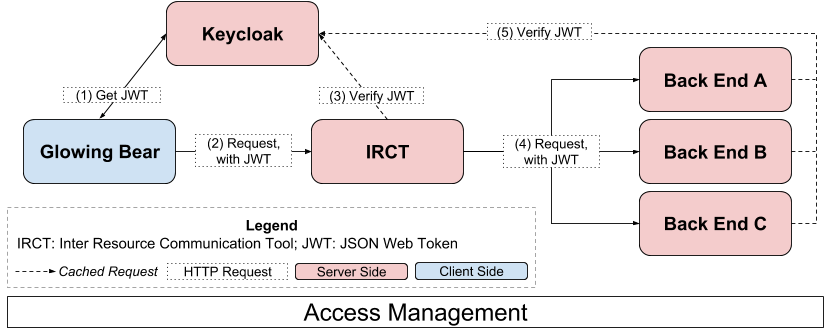
\includegraphics[width=1\textwidth]{figures/access_mgmt.png}
%     \caption{Diagram of the access management design.}
%     \label{fig:accessmgmt}
% \end{figure}


\subsection{Authorization}

% overview
Authorization management is about restricting access to data depending on the access level of the user.
With OIDC, the authorizations of an user are embedded as a \emph{claim} into the JWT by the identity provider.
While the authorizations are set at the identity provider, their enforcement are the responsibility of the client system, in this case tranSMART. 
Note that i2b2 and IRCT do not use the authorization capabilities of OIDC, only its authentication mechanism.

% authorization encoding
The standard does not specify a format for encoding authorizations, it is left at the client system discretion.
As Keycloak has its own format of authorization encoding, it also provides the ability to map authorizations to a specific format according to the client.
It is thus the responsibility of the administrator doing the deployment to make these two formats match by using the mapping capabilities of Keycloak.

% transmart/client authorizations enforcement
% todo?

\subsection{Implementation}

% \subsubsection{Keycloak}
% todo: add deployment and configuration of keycloak?

\subsubsection{Glowing Bear}

% add oidc support + http interceptor
Glowing Bear originally makes use of the client side of the OAuth2~\cite{oauth2} protocol for authorization with tranSMART. 
We thus modify it to use the OpenID Connect protocol.
To embed the JWT into the HTTP requests an interceptor is implemented. 
It intercepts all the requests made by Glowing Bear, examines it, and add in the headers the token if it is needed so that they are authenticated at the back end receiving the request.

\subsubsection{IRCT}

% RS256 implementation
In its original implementation IRCT supports only JWT with a \verb|HS256| signature, i.e. a shared-secret based signature. 
Because Keycloak does not support this type of signature, and because the standard recommends to use \verb|RS256| signature~\cite{todo}, we modify the IRCT implementation to do so. 
The support of \verb|RS256| signatures is added alongside \verb|HS256|, which instead of the shared secret needs as input the public signing keys of Keycloak.
The retrieval of those in the JWKS format is thus implemented, from an URL specified in the configuration.
The verification of the token is voluntarily incomplete: checking for the issuer and the client identifier is left as the responsibility of the back end system queried by IRCT.

\subsubsection{i2b2}

% oidc compat and parameters i2b2
i2b2 initially supports authentication with its own user management mechanism or through LDAP or NTLM directories.
We take advantage of the i2b2 Project Management (PM) cell ability to specify in the database the authentication mechanism to add the OpenID Connect implementation.
This allows users authenticated with OIDC to cohabit with users authenticated with the traditional i2b2 way.
This is done through the i2b2 PM parameters (as specified section~\ref{sec:bg-i2b2}), which can be applied either at user, cell or project level. 
They are the following:

\begin{itemize}
    \item token issuer (Keycloak instance URL)
    \item signing public keys URL (JWKS)
    \item client identifier
    \item field name in the JWT of the user's username
\end{itemize}

This last field is needed in order to be sure that the user account in the i2b2 database matches the user specified in the token, in order to enforce the authorizations.
Because there is no such thing as a standard username field, it needs to be specified by the configuration.

% how token is sent
The token is passed through the \verb|password| field of the i2b2 XML API (see appendix~\ref{sec:appendix-i2b2}).
This approach is not among the recommended ones, but it does not go against the OpenID Connect standard, and it simplifies greatly the implementation.


% todo ------- merge this:
% \subsection{Identity and Access Management}
% THIS IS FOR 3.1

% % auth with IRCT
% All requests made to IRCT with the PIC-SURE API must be authenticated with a JWT as explained section 


% % auth with data sources
% Because IRCT communicates with i2b2, it has to somehow be authenticated with it.
% We support two ways of doing so:
% \begin{itemize}
%     \item IRCT requests are authenticated against i2b2 as being the IRCT system
%     \item IRCT requests are authenticated as being from the requesting user in the client system
% \end{itemize}
% The first implies that IRCT must have a fixed set of credentials to authenticate against i2b2.
% This poses some obvious security problems, as this means that all users using the PIC-SURE API must have the same level of access.
% The second one, which we use in our solution, makes use of the user's JWT, 
% access mgmt / authorization handled by the data source, user must exisgt in data source

% matching users

% \subsubsection*{Implementation}
% - cors
% - token change type -> prev sec
% - i2b2 auth -> prev sec
% todo: mention the gb + transmart process, citation, to rely on what is existing already
% todo: gb screenshots

\section{Front End: Glowing Bear}
\label{sec:interoplayer-gb}

% overview
The front end we chose to use, Glowing Bear, is modified to support the PIC-SURE API in addition to the existing support of the tranSMART REST API v2.
This section describes the process of Glowing Bear with PIC-SURE only, as the support for tranSMART is preexisting.
For each part, we first describe the workflow in its final form, and then which implementation steps are taken to reach that stage.

\subsection{Initialization}

% configuration
The very first step is reading the configuration, which defines the mode in which the running instance is running: tranSMART or PIC-SURE; and the according authentication process to use.
It also allows to enable or disable certain features, according to the back end compatibility.
The features that can be controlled this way are:
\begin{enumerate*}
    \item query saving,
    \item data table,
    \item query subscription,
    \item data analysis,
    \item data export,
    \item observation count,
    \item variable selection,
\end{enumerate*}
which are all disabled when using PIC-SURE.

% login / pic-sure resource
After the configuration is loaded, Glowing Bear checks the validity of the token and redirects the user to the Keycloak login page if invalid or not present.
After the login is successful Glowing Bear gets the list of available resources with the PIC-SURE API and extracts the definition of the resource it is configured to use (see~\ref{sec:bg-picsure}).


\subsubsection*{Implementation}

% configuration
The following configuration options are added:
\begin{itemize}
    \setlength\itemsep{0em}

    % mode
    \item \verb|endpoint-mode|: use tranSMART or PIC-SURE mode
    \item \verb|picsure-resource-name|: PIC-SURE resource to use
    \item \verb|force-i2b2-nesting-style|: force the i2b2 AND/OR query format
    \item \verb|enable-greedy-tree-loading|: controls whether the tree of query terms should be loaded entirely during initialization \\

    % oidc
    \item \verb|authentication-service-type|: controls the type of authentication service used
    \item \verb|oidc-server-url|: URL of the OpenID Connect server
    \item \verb|oidc-client-id|: client identifier to use with the OIDC server \\
    
    % enable disable features
    \item \verb|show-observation-counts|: controls the display of the observation counts
    \item \verb|include-query-saving|: controls the use of the query saving feature
    \item \verb|include-data-table|: controls the use of the data table feature
    \item \verb|include-query-subscription|: controls the use of the query subscription feature
    \item \verb|include-variable-selection|: controls the use of the variable selection feature
    \item \verb|enable-analysis|: controls the display of the analysis tab
    \item \verb|enable-export|: controls the display of the export tab

\end{itemize}

% PIC-SURE resource implementation overview and resource fetching
We make the code agnostic to the differences between tranSMART and PIC-SURE except from a single service, the \emph{Resource Service}, which acts as an interface between the core Glowing Bear code and the API-specific code.
The use of one or another service is controlled by a configuration option.
We factor away into the \emph{API Endpoint Service} the methods that handle the HTTP calls from the \emph{tranSMART Resource Service}, so that they can be used in the newly implemented \emph{PIC-SURE Resource Service}.
At initialization this service fetches the definition of the PIC-SURE resources available, and implements the PIC-SURE API calls.

% todo: talk about resource def model and others?

\subsection{Query Terms Tree}
\label{sec:design-tree}
% todo: relationship: child and modifier, see how much to put here and how much in background

% initialization & browsing
Right after Glowing Bear is fully initialized the tree of query terms is loaded.
As PIC-SURE supports only node-per-node loading, just the root nodes are loaded. 
This behavior is controlled by a configuration option.
For this reason, the free-text search in the tree can not be used and the auto-completion feature in the query construction component is degraded and only has the already-loaded nodes.
Then as the user expands the nodes in the tree, calls are made to the back end to dynamically load the children nodes.

% tree structure
Each node in the tree in characterized by a unique path, which for PIC-SURE on i2b2 has the following format:
\begin{verbatim}
    /<data source name>/<i2b2 project name>/<category>/.../<concept>/
\end{verbatim}
When displaying the tree, we omit the first element of the tree (\emph{PIC-SURE resource name}) as it is constant during the runtime, specified by the configuration.

% node content
Tree nodes each contain the information needed to be used as a query term.
They can be of three types: \emph{concept}, \emph{modifier}, \emph{study}, or \emph{unknown}.
An unknown type node is not queryable. 
A study type node is only used by tranSMART.
A modifier type node is applied as a constraint to a concept.
The queryable nodes in i2b2 are all concepts, and are themselves subdivided in several types:
\begin{itemize}
    \setlength\itemsep{0em}
    \item \emph{Simple}: simple concept with no associated value
    \item \emph{Categorical}: concept with a categorical (i.e. enumerated) value
    \item \emph{Numerical}: concept with a numerical value
    \item \emph{Text}: concept with a free-text value
\end{itemize}
Each of those types is mapped to the appropriate user interface component, for taking the user input.
This component is displayed in the query construction component, after the tree node is drag-and-dropped from the tree.
Additionally the nodes have the information about whether or not they may have children, i.e. if they are leaves in the tree.


\subsubsection*{Implementation}

% loading refactor
Originally Glowing Bear supports only a greedy loading method, as in the whole tree is loaded at initialization.
Because PIC-SURE does not support this, at least not with acceptable performance, we refactor the \emph{Tree Node Service} to load at initialization time only the root node, if specified in the configuration.
Then we add in the \emph{Tree Node Component}, which displays the tree in the UI, the ability to load dynamically the children nodes when the user expands a tree node with missing children.

% tree node type
The original tranSMART tree node implementation represents tree nodes without typing, i.e. generic objects.
To improve the code quality and enforce a common structure between the two API implementations, we create a new \emph{Tree Node Model}.
We modify the tranSMART and create the PIC-SURE API implementations so that they both produce the same \emph{Tree Node Model}.
Among the concept types originally supported, we add the types \emph{categorical option}, \emph{text}, \emph{high dimensional} and \emph{simple}.
These cover both the new i2b2 types, and a regrouping of tranSMART types for more clarity.


\subsection{Query Construction}

% intro
The user constructs his query by drag-and-dropping query terms from the tree to the query construction component.
As the user do so, Glowing Bear might request to the back end additional information on the query terms.
Once done, and before submitting to the back end, this query is mapped to the PIC-SURE query format.

\subsubsection{Query Terms Metadata}

% intro and request
When a query term is dropped into the query construction component, a dedicated sub-component is created.
This sub-component when initialized will, according to the query term type, make a request to the back end using a tree node call with the \verb|AGGREGATE| relationship, on the term that is about to be used in the query.
With an i2b2 resource, this call is used for \emph{categorical} query terms types, as i2b2 does not have support to return aggregate values of numerical or date terms.

% answer
The answer is a usual PIC-SURE tree node answer, with additional metadata containing the categorical values.
These are then used by the sub-component to be displayed to the user.
Example of such an answer:

\begin{samepage}
\begin{verbatim}
{
    "pui": "/<concept path>/",
    ...
    "attributes": {
        ...
        "aggregate.categorical.0": "<categorical value 0>",
        "aggregate.categorical.1": "<categorical value 1>",
        ...
}
\end{verbatim}
\end{samepage}


\subsubsection{Generation of PIC-SURE query}
\label{sec:gb-query}

\paragraph{Data Types}
A query is a set of constraints, expressed as a list of \emph{where clauses} as explained in \ref{sec:bg-picsure}.
As each tree node is associated to a PIC-SURE data type like explained in section~\ref{sec:design-tree}, we know through the resource definition what predicates can be applied on them.
For an i2b2 resource, here follows the data types and corresponding predicates:
\begin{itemize}
    \setlength\itemsep{0em}

    \item \emph{Simple} concept: \verb|CONTAINS|, \verb|CONSTRAIN_DATE| and \verb|MODIFIER| predicates
    \item \emph{Categorical}, \emph{Numerical} and \emph{Text} concept: the above and \verb|CONSTRAIN_VALUE|
\end{itemize}

\paragraph{Predicates}
Some predicates takes values as input:
\begin{itemize}
    \setlength\itemsep{0em}

    \item \verb|CONSTRAIN_VALUE|:
    \begin{itemize}
        \item \verb|OPERATOR|: the operator to apply on the value 
        \item \verb|CONSTRAINT|: the value of the constraint
        \item \verb|UNIT_OF_MEASURE|: optionally the measure unit of the value
    \end{itemize}
    
    \item \verb|CONSTRAIN_DATE|:
    \begin{itemize}
        \item \verb|FROM_INCLUSIVE|, \verb|TO_INCLUSIVE|: if the to / from date is inclusive
        \item \verb|FROM_DATE|, \verb|TO_DATE|: date constraint boundaries
        \item \verb|FROM_TIME|, \verb|TO_TIME|: if the to / from constraint should be applied on the start or end date of the observation
    \end{itemize}
    
    \item \verb|CONSTRAIN_MODIFIER|:
    \begin{itemize}
        \item \verb|MODIFIER_KEY|: key of the modifier to be applied on the concept
    \end{itemize}
\end{itemize}

\paragraph{Example}
Assembling those together, a \emph{where clause} based on a value would be similar to the following:
\begin{samepage}
\begin{verbatim}
[{
    "field": {
        "pui": "/resource/project/laboratory/biochemistry/Creatinine (mg per dL)/",
        "dataType": "CONCEPT_NUMERIC"
    },
    "predicate": "CONSTRAIN_VALUE",
    "fields": {
        "OPERATOR": "GT",
        "CONSTRAINT": "4,2"
    }
}]
\end{verbatim}
\end{samepage}

\paragraph{Combination of query terms}
While tranSMART supports full freedom in the combination of query terms, i2b2 is restricted to the following format:
\begin{verbatim}
    (A OR B OR ...) AND (C OR D OR ...) AND ...
\end{verbatim}
That is, blocks of query terms linked by an \verb|AND|, themselves linked by an \verb|OR|.
The restriction to this format is controlled by the configuration, and if enabled the user if forced to respect it.
In the PIC-SURE API, this translates to setting accordingly the \emph{logical operator} as such:
\begin{samepage}
\begin{verbatim}
[
    { 
        <where clause definition>,
        "logicalOperator": "AND"
    }, {
        <where clause definition>,
        "logicalOperator": "OR"
    },
    ...
]
\end{verbatim}
\end{samepage}

% todo: cover the negation? not actually used


\subsubsection{Implementation}
% todo: is there more than that?

% query metadata
The mechanism to request metadata about a query term to the back end is preexisting.
As such we implement the call in the \emph{PIC-SURE Resource Service} that returns the specific model that Glowing Bear expects to populate its data structures for the display and selection of the categorical variable.

% query construction
The whole process of generating queries in the PIC-SURE format are implemented in a new utility class \emph{PIC-SURE Constraint Serializer}.
Models representing the \emph{where clauses} are implemented, and the serializer is responsible to produce those, based on the Glowing Bear internal models that represent the query.

% combination
In order to restrict the format of the queries to the i2b2 format, a configuration option is added.
If enabled, the component holding the combination of query terms enforce this restriction.
The first level of nesting is always an \verb|AND|, the second level always an \verb|OR|, and no more levels are allowed.


\subsection{Query Request & Result Retrieval}
\label{sec:interoplayer-gb-results}

% intro
After constructing the query as previously described, Glowing Bear submits the query to the back end using the \emph{PIC-SURE Query Service}.
At this stage, we are interested only in the result patient count of the query to be displayed to the user, which is what is requested in the query.

\paragraph{Query Request}
When using only inclusion criterion, a single query is submitted as expected. 
The count returned is displayed as it is to the user.
However when using both inclusion and exclusion criterion, two query requests are actually submitted:
\begin{itemize}
    \setlength\itemsep{0em}

    \item Query 1: \verb|<inclusion criterion>|
    \item Query 2: \verb|<inclusion criterion> AND <exclusion criterion>|
\end{itemize}

Note that in the second query, the exclusion criterion is not negated.
Making two separate queries allows to display slightly more detailed counts to the user:
\begin{itemize}
    \setlength\itemsep{0em}

    \item Inclusion count: \verb|<Q1 count>|
    \item Exclusion count: \verb|<Q2 count>|
    \item Query total count: \verb|<Q1 count> - <Q2 count>|
\end{itemize}


\paragraph{Result Retrieval}
Due to the asynchronous nature of the PIC-SURE queries, the request does not include the actual result, but the identifier of the result.
Using this identifier, Glowing Bear regularly polls the back end using the \emph{PIC-SURE Result Service} to inquire about the result status.
This status can take several values:
\begin{itemize}
    \setlength\itemsep{0em}

    \item \verb|RUNNING|: the query is still running, the regular polling continues
    \item \verb|AVAILABLE|: the query has successfully finished and the result can be requested
    \item \verb|ERROR|: the query is in error state, the polling stops and the user is informed of the error message that comes along
\end{itemize}

When the result becomes available, it is requested using the same identifier and then displayed.


\subsubsection*{Implementation}

The implementation of this part is made in the Glowing Bear \emph{PIC-SURE Resource Service}, orchestrated from a single method as the core code expects synchronous count results from the query.
The result retrieval is configured to poll every second the back end for the result status, and waits up to one minute.
If after one minute the result is not available, it is considered as failed.

Additionally, because i2b2 supports only patients count and no observations count, the display of this value is disabled through the configuration.


% todo: mention the i2b2 process and all from paper

\section{PIC-SURE to i2b2 API Translation}
\label{sec:interoplayer-picsure}

% intro
On the back end side, to provide an interoperability layer with i2b2 and later more systems, we use IRCT~\cite{todo} (Inter-Resource Communication Tool).
IRCT implements the PIC-SURE API, which is used by Glowing Bear.
Behind that it can support a multitude of systems, but we focus here on the support of i2b2.

% overview
This section covers the process of API translation happening in IRCT, from the PIC-SURE API to the i2b2 API.
We go over the full query process: browsing through query terms, executing a query and getting back its results.


\subsection{Query Terms Tree}

\subsubsection{Tree Structure and Nodes Relationships}

% tree structure and root
Query terms in are exposed through a tree to client systems.
Each node in the tree is uniquely identified by a path, with at its root the different data sources available in the instance.
When a client requests the children of the root path \verb|/|, the nodes returned correspond to the configured data sources in the instance.
Below this root level, the tree is data source implementation-dependent.
We review here the tree of an i2b2 data source.

% tree browsing
The data sources tree structure is based on \emph{relationships} between nodes.
The most obvious relationship is the parent / child / sibling: based on a tree node, a client can requests its \emph{children}, \emph{parent} or \emph{sibling} nodes.
This allows the client system to browse the tree in an iterative fashion, which is what happens with i2b2.
I2b2 itself already exposes a tree, so the mapping of the tree is one-to-one below a certain level:
\begin{verbatim}
    /<data source name>/<i2b2 project name>/<i2b2 root node (category)/<i2b2 tree>/
\end{verbatim}
Note that it is not possible to use query terms coming from different data sources at same time, or in the case of i2b2 from different projects.

% aggregate
On top of the previously mentioned standard relationships, a data source implementation can declare additional ones, which can be seen as adding a dimension to the tree.
We exploit here this possibility in order to expose aggregate data about the nodes.
Here we add an \emph{aggregate} relationship to the \emph{categorical} nodes, which is exposed the client system.
As such the client system knows about this possibility, and can request the aggregate values of node, in this specific case the values this categorical query term can take.

% list of relationships supported by i2b2
The relationships exposed by an i2b2 data source tree are:
\begin{itemize}
    \item \emph{Child}: returns the children node 
    \item \emph{Modifier}: returns the modifiers associated to the requested tree node
    \item \emph{Aggregate}: returns the aggregate data of the tree node (example: values of a categorical query term)
\end{itemize}


\subsubsection{Tree Nodes as Query Terms}

% link tree node - query term
To determine how tree nodes can be used as query terms, we do the following.
Each node of the tree can declare a type. 
If the node does not have a type, it is not queryable and is a simple "container" node.
When the node has a type it can be use used as a query term with some predicates, and each predicate declares in the data source implementation which node types it supports.
So we need to 
\begin{enumerate*}
    \item translate correctly the i2b2 node types into PIC-SURE node types
    \item declare predicates that support those types
\end{enumerate*}

% declaring types
The types can be defined by the data source implementation, or be one of the primitive types offered by IRCT.
With the i2b2 implementation, we do not use the primitive types, only the ones we define:
\begin{samepage}
\begin{itemize}
    \item \verb|concept|: simple query term, maps to the \emph{simple} GB types
    \item \verb|concept_numerical|: query term with numeric value, maps to \emph{numerical} GB type
    \item \verb|concept_enum|: query term with categorical value, maps to \emph{categorical} GB type
    \item \verb|concept_string|: query term with free-text value, maps to \emph{text} GB type
\end{itemize}
\end{samepage}

% todo: predicates mapping??

\subsubsection{Implementation}

% data type
Browsing the i2b2 ontology tree is already implemented in IRCT, we enhance it with some features that we need.
The specific i2b2 data types listed before are implemented, and the extraction of those types from the i2b2 ontology tree as well.
We also implement adding the relationships \emph{child} and \emph{aggregate} to the tree nodes if they need to.
The i2b2 data source definition is modified accordingly.
% todo: modifier?

% aggregate
Support for the \emph{aggregate} is implemented by making an ontology request to i2b2, and parsing the XML metadata associated to the node that contain this information, to embed the categorical values in the tree node.


\subsection{Query Translation}
\label{sec:interop-layer-query-translation}

Here we show the process of translating a query from the PIC-SURE API format to the i2b2 API format.

\subsubsection{Query Structure Translation}

% i2b2 generality, terminology
Recall that all the query terms are represented in the PIC-SURE API by a \emph{where clause}.
In the i2b2 terminology, a query term is an \emph{item}, and a group of query terms linked by an \verb|OR| is a \emph{panel}.
The \emph{panels} are linked together with an \verb|AND|.
The translation process from the PIC-SURE to the i2b2 API iterates over all the \emph{where clauses}, translate them into an i2b2 \emph{item}, and assemble those \emph{items} appropriately into \emph{panels} according to the PIC-SURE logical operator used.

% pic-sure query example
\begin{samepage}
See below an example of a PIC-SURE query, with query terms \verb|A|, \verb|B|, \verb|C| and \verb|D|:
\begin{verbatim}
[
    { 
        <A>
    }, {
        <B>,
        "logicalOperator": "OR"
    }, {
        <C>,
        "logicalOperator": "AND"
    }, {
        <D>,
        "logicalOperator": "OR"
    }
]
\end{verbatim}
\end{samepage}

% abstracted
\begin{samepage}
This query can be abstracted as seen below.
Here a query term denoted by~\verb|*| is an \emph{item}, and a block of query terms denoted by~\verb|---| is a \emph{panel}.
\begin{verbatim}
     *    *       *    *
    (A OR B) AND (C OR D)
    --------     --------
\end{verbatim}
\end{samepage}

% i2b2 format
\begin{samepage}
This query would be translated into the following i2b2 XML query format:
\begin{verbatim}
    <panel>
        <item>A</item>
        <item>B</item>
    </panel>
    <panel>
        <item>C</item>
        <item>D</item>
    </panel>
\end{verbatim}
\end{samepage}


\subsubsection{Query Terms Translation}

When translating a query term into and i2b2 \emph{item}, some additional processing might be needed according to the predicate used.
It is not the case for the simple \verb|CONTAINS| predicate, which is straightforwardly translated using the path in the i2b2 ontology tree.
For the others, the additional information is added to the item:

\begin{samepage}
\begin{itemize}
    \item \verb|CONSTRAIN_MODIFIER|: on the item is added the path of the applied modifier in the ontology tree
    \item \verb|CONSTRAIN_DATE|: on the item is added the dates and parameters specified by the querier
    \item \verb|CONSTRAIN_VALUE|: on the item is added the value and parameters specified by the querier
\end{itemize}
\end{samepage}


\subsubsection*{Implementation}

The translation of queries is left mostly untouched from its original implementation, except from the support of query terms negation that is implemented.


\subsection{Results Management}

After making the query request, IRCT registers in its own database the query with an identifier that encodes the different corresponding identifiers on the i2b2 side:
\begin{verbatim}
    <i2b2 project id>|<i2b2 query id>|<i2b2 result id>
\end{verbatim}

Using those i2b2 identifiers IRCT is able to request to i2b2 the status of the query.
Once the query is over and successful, its patient count results are retrieved from i2b2 and stored in the IRCT database.


\subsection{Miscellaneous implementation tasks}

% hibernate change
While IRCT uses Hibernate~\cite{todo} to abstract away the SQL database used, in our case using PostgreSQL does not work as the default SQL table names use some reserved keywords.
To counter this we use the Hibernate feature that allows to add a specific prefix to the table names.

% sql functions
Configuring an i2b2 data source to be used in IRCT requires to add a specific set of data in the PostgreSQL database.
To do so, we implement a PL/pgSQL function that can be called with the appropriate parameters to add an i2b2 resource.

% cors
Web browsers block by default web requests made to other web site than the web site it originate from, as a security feature.
This can circumvented by using the Cross-Origin Resource Sharing (CORS)~\cite{todo} standard that modern web browsers implement.
CORS allows web pages to make web requests to web site other than the web site from which the script is executed, but only if the web service serving the request explicitly allows the web site from which the request originates.
This is checked automatically by the browser, which before making an actual HTTP request, will make an \verb|OPTION| HTTP request to the web service to get the list of domains allowed to make requests.
This feature is not initially implemented by IRCT.
We implement it by allowing unauthenticated HTTP \verb|OPTION| requests, and by embedding the appropriate headers into the answer.


\chapter{Privacy-Preserving Cohort Exploration}
\label{sec:medco}


% thesis: medco subject to previous work of author, modified as such... (check out paper for more info)

% intro
% We adapt and integrate a privacy-pres
% Building on top of the interoperability layer described in the last section, we achieve in this section the ability to do cohort exploration with our system in a privacy-preserving way.

% explain what is medco, several nodes, etc.
\section{Detailed Workflow}

We show here the detailed workflow of our system when using MedCo.
The first two step \ref{enum:wf-interop-login} and \ref{enum:wf-interop-login} from the interoperability layer (section~\ref{sec:interoplayer-wf}) are the same, and the following differs:

\begin{enumerate}
\item \textbf{User Login}:
T

\end{enumerate}

% todo: put medco more detailed diagram

\begin{itemize}
\item \textbf{Query Construction}:
The user browses the tree of query terms and uses them to construct a query corresponding to a patient set.
When adding a term into the query panel, Glowing Bear might, according to its type, make a background request to fetch the term metadata, which is the case for example for categorical or numerical terms.
The user then optionally sets value(s) to the query term.

\end{itemize}

mention about edco resource ahs to be implemented: in two parts mainly: tree and querhy

result is same as i2b2
tree is same as i2b2 almost / converter for types added

medco builds on i2b2, as a cell in hive 

uses i2b2 api with some fine tuning 
(result in json show it 
encrypted key show it

medco cell processing show it : encrypted -> tagged)

\section{Glowing Bear Query Construction}
say it is inherated from i2b2 / 
data types new
% assumptions made:
% - ontologies match exactly
% - authentication: user exists in the 3 pms?


% for implementation of medco res. interface / extends though

\begin{itemize}
    \item tree browsing, number to encrypt in the tree
    \item same as described before, with a special data type and predicate used
    \item encryption of terms 
    \item format of encrypted terms
\end{itemize}

% gen temporary priv / pub pair of keys for user, in impl: hardcoded
% encrypt with group.toml file from config the values to be sent
% decrypt w/ priv key the results

\subsection*{Implementation}

- npm package
- key gen


\section{IRCT Query Broadcast}

% intro
After Glowing has submitted to IRCT the query through the PIC-SURE API, IRCT invokes the MedCo data source implementation to run the query with the MedCo nodes.
Running the query with the MedCo nodes uses the i2b2 XML API, but do not reuse the i2b2 data source implementation like with the tree browsing, due to fundamental differences in how the query is executed.

% threading
The process to generate the query in the i2b2 XML API format is the same as i2b2, described section~\ref{sec:interop-layer-query-translation}, even though the paths of the queried items are encrypted values.
However the submission of the query to i2b2 is different, as the query has to be submitted to all the MedCo nodes simultaneously.
This is needed as the MedCo nodes later need to synchronize between to perform some collective cryptographic operations.


% medco resource, where? should be before

\subsection*{Implementation}

% threading
We implement the part of the PIC-SURE data source implementation for MedCo that handles the querying of the data source.
To implement the simultaneous querying of the MedCo nodes, we use as many threads as there are nodes and execute them at the same time. 
We use a \emph{count down latch} to synchronize the threads together and wait on their completion.
After a set amount of time without answer from the MedCo nodes, they timeout.

% shrine drop
The query is submitted directly to the MedCo nodes. 
This is different from the original MedCo behavior that relies on SHRINE~\cite{todo} to do so.
In this previous implementation, the query was submitted to a single SHRINE node, and only after the query was broadcasted to the MedCo nodes.
Here this broadcaster role is taken by the PIC-SURE data source implementation of MedCo.
The reasoning bypassing SHRINE is that it is a multi-components software, that is complicated to set up and deploy, and is expensive to maintain.
Moreover it was not bringing a significant added value to MedCo.

% ontology
Doing so, we lose a feature offered by SHRINE, which is the ontology translation that SHRINE operates, between a common network ontology and a local i2b2 ontology.
This is not a big problem, as anyway the mapping between the network and common ontology needed to be made and maintain manually in SHRINE.
Also this feature is not used in MedCo for the encrypted terms.
It implies though that the ontologies between the different MedCo nodes have to be maintained identical, at least for the ontologies meant to be queried through MedCo.

\section{MedCo Query Processing}
\begin{itemize}
    \item summarize how medco works
    \item modifications made: shrine drop, ?
\end{itemize}

secure shuffle with aaaaaaa

% each ontologiy at each site has 2 ontologies, clear and not clear, explorable by client or not 
% schemas "medcon otology" " i2b2metadata_i2b2"


% no repeat of what medco process is doing and already described in paper, cite it in detail though


\section{Glowing Bear Result Processing}

% intro
Following the same process as i2b2 described in section~\ref{sec:interoplayer-gb-results}, the results of the query are retrieved from IRCT.
The difference here is in the format of the results, as they are encrypted with the public key $P_k$ sent along the query.

% result format
There is one result per MedCo nodes.
According to access level of the user, it is possible to identify which result is coming from which node, or the result were securely shuffled between the nodes.
The format of the result is a JSON string with the following format:

\begin{verbatim}
{
    "pub_key": "<public key used>",
    "enc_count_result": "<result encrypted with public key>",
    "times": {
        <breakdown of time measurements>
    }
}    
\end{verbatim}

% decryption
All the encrypted results are then decrypted using the secret private key $p_k$, summed together, and displayed to the user using the same process as for i2b2.
Additional information, containing the more detailed breakdown of results per node, is also displayed.


\subsection*{Implementation}

% decryption
A modification is made in the Glowing Bear PIC-SURE results processing to identify correctly when encrypted results are fetched, and extract them.
Decryption of the results are made using the cryptography library previously described, and the private key corresponding to the public key used.

% breakdown component
A new module is implemented in order to display the detailed breakdown of the MedCo query.
It appears as a tab when Glowing Bear detects the presence of MedCo results, and displays the count breakdowns and times measurements from the nodes.

\chapter{System Evaluation}

% todo: this section should show how the requirements are met

\begin{itemize}
    \item goals: meet the requirements
\end{itemize}

\section{Experiments}
% todo: overhead compared to orig GB

% - questions to be answered: overhead of this new implementation + security of the whole system
% - exp. setup
% - experiments
% - summary

\begin{itemize}
    \item i2b2 query times vs picsure+i2b2 query times (overhead)
    \item medco query times with pic-sure vs previously with shrine (refer to the paper)
    \item experimental setup & methodology
\end{itemize}

% put that or not? see if there is sth to say
\section{Security Analysis}
\begin{itemize}
    \item security analysis
    \item threat model
\end{itemize}

% - : i2b2 pws in clear in xml changed 
% where are other problems?
% how to do an analysis: cehck out owasp?
% threats models: https://www.owasp.org/index.php/Testing_Guide_Introduction#Threat_Modeling
% https://www.owasp.org/images/1/19/OTGv4.pdf ?

% (incl. medco threat model in there)
% have zones for data and such
% including communications, systems

% authorizations

% need for https comms (proxied here)


\section{Requirements Fulfillment}
\begin{itemize}
    \item take list of requirements and explain how they are met
\end{itemize}

\section{Discussion}
\begin{itemize}
    \item limitations
\end{itemize}

\chapter{Conclusion}
% not just summary: insightful conclusion

\section{Future Work}

\begin{itemize}
    \item additional pic-sure resources: HAIL, ODSY OMOP
    \item for HAIL: the R connector through PIC-SURE, work of Denise
    \item missing features: query saving, data extraction
\end{itemize}

% HAIL / R / PIC-SURE: https://www.ncbi.nlm.nih.gov/pubmed/29267850
% checkout/mention more general systems: scidb / elasticsearch / olap-mdx (mdx is the query language, olap the model)-could be envisioned to be supported thorgh pic sure --> go to future work

% add blockchain auth (gb)

% ---- appendices ----
\newpage
\appendix
\chapter{Online Resources}
% github / docker cloud / npm / repos / ...0
%unlynx-crypto-js-lib -> medco-js-lib?
% todo: acronyms in appendix
\chapter{Docker-Based Testing Infrastructure}
\label{sec:docker}

% This appendix describes the docker-based infrastructure put in place to test the systems.

\section{Docker Images}
\label{sec:docker-images}


% \subsection{Deploying Original Components}
% % todo: transmart 16.2?
% % todo: versions to be used

% First of all we are compiling, setting up and deploying all the building blocks of the solution: Glowing Bear, IRCT, tranSMART 17.1, i2b2, SHRINE.
% The exhaustive information about the deployments using Docker can be found in appendix~\ref{sec:docker-images}.
% These components require some servers that are deployed with Docker: WildFly (application server), PostgreSQL (database server), lighttpd (web server)

% % GB
% We are deploying Glowing Bear from the sources using the Angular command \verb|ng serve|, which is practical for development.
% For production deployment it is deployed through the web server.
% The version used is branched off the development branch \verb|table|, which is the most up to date branch at the time of the writing, and is regularly rebased on this same branch.
% It is configured to use the locally deployed instance of back end components.

% % todo: put in annex for docker deployment, also db
% Keycloak is deployed as an OpenID Connect server using its official Docker image that sets up a working instance.
% It uses the same PostgreSQL database that other deployments are using.
% The version used is 3.4.3.
% It is configured with a local user data source managed by itself, and one client for each back end that will use this instance.

% % IRCT
% IRCT is compiled from sources and deployed using Docker.
% The version used is a fork of the latest version on the master branch of the repository. 
% It is regularly rebased to keep track of the changes.
% It is configured to use one local instance of each type of supported back end systems: i2b2, tranSMART 17.1, SHRINE.
% The configuration is done through the local PostgreSQL database.

% % i2b2
% I2b2 is compiled from sources and deployed using Docker.
% The version used is TBD.
% The Spring configuration files and test data comes from the demo dataset that is provided with i2b2, and allows to have a demonstration running instance, done through the local PostgreSQL database.

% % tranSMART 17.1
% tranSMART 17.1 is compiled from sources and deployed using Docker.
% The version used is TBD.
% The configuration is done through a grails configuration file, and some test data is loaded in the local PostgreSQL database used.

% % SHRINE
% First step of the SHRINE deployment it to modify the existing i2b2 deployment.
% Its demo data (loaded in PostgreSQL) is duplicated three times, to replicate (with the appropriate configuration) three different instances of i2b2 (but served through the same web service).
% Then three instances of the SHRINE web services are deployed: this corresponds to a setting where the SHRINE network has three nodes.
% It is compiled from sources and deployed using Docker. 
% The version used is TBD.
% It is configured through simple configuration files.
% The SHRINE instances use a deployment of the MySQL database server for their data.
% The SHRINE webclient is served by the web server.


%mention keycloak + postgresql, not from scratch images

\subsection{i2b2}

\subsection{tranSMART 17.1}

\subsection{IRCT}

\subsection{i2b2 MedCo}
% todo: medco docker create ont schema medco


% This section describes the different Docker images of the infrastructure.

% \subsection{WildFly Application Server}

% \begin{itemize}
%     \item Ports exposed
%         \begin{itemize}
%         \item 8080: deployments endpoint
%         \item 9990: WildFly management interface
%         \end{itemize}
        
%     \item Volumes
%         \begin{itemize}
%         \item \verb|/opt/jboss/wildfly/standalone/deployments/|: deployment folder of WildFly
%         \item \verb|/opt/jboss/wildfly/standalone/configuration/|: configuration folder of WildFly
%         \item \verb|/opt/jboss/.grails/|: Grails configuration folder (for user \verb|jboss|)
%         \end{itemize}
% \end{itemize}

% This sets up a working WildFly server and install several tools used to build from source the different WARs that are deployed.
% Upon initial creation of the container there is no deployment, they are built on demand with the help of the build scripts that are shipped in the image.
% With the container running, run the following command to build a deployment: 

% \begin{verbatim}
% docker exec -it <container_name> build-war.sh <deployment_name>
% \end{verbatim}

% When running with the default docker-compose configuration, the name of the container would be \verb|deployments_wildfly-server_1|.
% Below are described the different deployments that can be built.

% \subsubsection{i2b2}
% Deployment name: \verb|i2b2|, URL exposed: \verb|/i2b2/|

% The i2b2 WAR is actually a deployment of Axis2. Within this deployment, all the i2b2 cells are deployed as AAR files (Axis2 Archive):

% \begin{itemize}
%     \item \verb|CRC|: Clinical Research Chart (data repository)
%     \item \verb|ONT|: Ontology management
%     \item \verb|PM|: Project Management (authentication and authorization)
%     \item \verb|WORK|: Workflow management (query, result sharing)
%     \item \verb|FR|: File Repository
%     \item \verb|IM|: Identity Management
% \end{itemize}

% \subsubsection{IRCT}
% Deployment name: \verb|irct|, URL exposed: \verb|/IRCT-CL/|

% Note that before you can build the IRCT deployment, i2b2 should have been built before (in order to deploy the JDBC drivers), and the database should up and initialized correctly.
% This is due to the fact that IRCT uses Hibernate to handle its data storage in the database, and when ran it will validate and update if necessary the database schema.
% To resolve an incompatibility of IRCT using Hibernate with the use of PostgreSQL, Hibernate is configured to add a prefix to all of the tables.

% \subsubsection{tranSMART 17.1}
% Deployment name: \verb|transmart-17.1|, URL exposed: \verb|/transmart-17.1/|

% % todo: a few lines


% % todo: deployments to add: tranSMART 16.2, SHRINE, MedCo

% \subsection{PostgreSQL Database Server}

% \begin{itemize}
%     \item Ports exposed
%         \begin{itemize}
%         \item 5432: PostgreSQL port
%         \end{itemize}
        
%     \item Volumes
%         \begin{itemize}
%         \item \verb|/var/lib/postgresql/data/|: PostgreSQL database files
%         \end{itemize}
% \end{itemize}

% This sets up a working PostgreSQL server and install several tools needed by the loading scripts that are ran upon the first run of the container.
% These scripts are copied in the \verb|/docker-entrypoint-initdb.d| folder.

% Below is an overview of the databases created.

% \subsubsection{i2b2}
% Contains the i2b2 database schemas for all the cells and the default demo data.

% \subsubsection{irct}
% Contains a snapshot of the IRCT database structure (that is updated as needed by Hibernate), and the resources information used by IRCT to connect to the resources:

% \begin{itemize}
%     \item \verb|i2b2-local|: the local i2b2 instance
% \end{itemize}

% \subsubsection{transmart\_17\_1}
% Contains the structure and some default test data for tranSMART 17.1.
    
\subsection{Lighttpd Web Server}

% \begin{itemize}
%     \item Ports exposed
%         \begin{itemize}
%         \item 80: HTTP port
%         \end{itemize}
% \end{itemize}

% This sets up a working Lighttpd server with PHP and install several services:
% \begin{itemize}
%     \item \verb|/phppgadmin/|: phpPgAdmin PostgreSQL management tool
%     \item \verb|/i2b2-client/|: the i2b2 webclient, using the local i2b2 instance
%     \item \verb|/i2b2-admin/|: the i2b2 admin tool, managing the local i2b2 instance
% \end{itemize}


\section{Docker-Compose Run Configuration}
% A default \verb|docker-compose.yml| is provided and works out of the box to create and deploy the images described section~\ref{sec:docker-images}.
% It creates a network to allow all the containers to communicate, exposes on the host the same ports as exposed by the container, and maps the WildFly volumes to directories alongside the Dockerfile.
% It does not require additional argument to be built and upped with the default configuration.

\chapter{APIs Usage Examples}

This appendix gives examples on how to use some APIs that are referred to in the thesis.

\section{tranSMART REST API v2}

% todo: make better and more
% todo: contains REAL examples (i.e. real response)
\paragraph{List of studies}
The list of available studies is requested:
\begin{verbatim}
GET /v2/studies
\end{verbatim}

Response:
\begin{verbatim}
{
  "studies": 
  [
    {
      "id": -20,
      "studyId": "CATEGORICAL_VALUES",
      "bioExperimentId": -10,
      "dimensions": 
      [
        "concept",
        "patient",
        "study"
      ]
    },
    ...
}
\end{verbatim}

\paragraph{Query Terms Tree}
The tree of the queryable terms is recuperated, with a depth of 2:
\begin{verbatim}
GET /v2/tree_nodes?root=&depth=2&tags=true
\end{verbatim}

Response:
\begin{verbatim}
{
  "tree_nodes":
    [
      {
        "name":"Vital Signs",
        "fullName":"\Vital Signs\",
        "name":"Vital Signs",
        "type":"UNKNOWN",
        "visualAttributes": ["FOLDER","ACTIVE"], 
        "children": [
          {
            "name":"Heart Rate",
            "fullName":"\Vital Signs\Heart Rate\",
            "conceptCode":"VSIGN:HR",
            "conceptPath":"\Vital Signs\Heart Rate\",
            "name":"Heart Rate",
            "type":"NUMERIC",
            "visualAttributes":["LEAF","ACTIVE","NUMERICAL"],
            "constraint": {
              "type": "concept",
              "conceptCode": "VSIGN:HR"
            }
          }
        ]
      },
      ...
    ]
}
\end{verbatim}

\paragraph{Saved Queries}
The list of previously saved queries is retrieved:
\begin{verbatim}
GET /v2/queries
\end{verbatim}

Response:
\begin{verbatim}
{
  "id": 1,
  "name": "testquery",
  "patientsQuery": {
    "constraint": {
      "args": 
      [
        {
          "conceptCode": "birthdate",
          "conceptPath": "\Demographics\Birth Date\",
          "fullName": "\Projects\Survey 1\Demographics\Birth Date\",
          "name": "Birth Date",
          "type": "concept",
          "valueType": "DATE"
        },
        {
          "studyId": "SURVEY1",
          "type": "study_name"
        }
      ],
      "type": "and"
    },
    "dimension": "patient",
    "type": "subselection"
  },
  "observationsQuery": {
    "data": [ ]
  },
  "apiVersion": "2.0",
  "bookmarked": false,
  "createDate": "2018-03-11T15:30:07Z",
  "updateDate": "2018-03-11T15:30:07Z"
}
\end{verbatim}


\paragraph{Query}

\begin{verbatim}
POST /v2/observations/counts_per_study_and_concept

{
  "constraint": {
    "type": "or",
    "args": [
      {
        "type": "subselection",
        "dimension": "patient",
        "constraint": {
          "type": "and",
          "args": [
            {
              "type": "concept",
              "conceptCode": "birthdate"
            },
            {
              "type": "study_name",
              "studyId": "SURVEY1"
            }
          ]
        }
      },
      {
        "type": "subselection",
        "dimension": "patient",
        "constraint": {
          "type": "and",
          "args": [
            {
              "type": "concept",
              "conceptCode": "O1KP:CAT1"
            },
            {
              "type": "study_name",
              "studyId": "ORACLE_1000_PATIENT"
            }
          ]
        }
      }
    ]
  }
}
\end{verbatim}

\subsection{Glowing Bear Workflow}
calls:
--- init step 0
1. /studies: list of studies, displayed under "Public Studies", some under "Private Studies" (distinction how??), and more, but how exactly are they mapped to the tree?

2. --> they are mapped with call to /tree\_nodes?root=\\ => each of the concept has a studyId to do the mapping
--> call to /tree\_nodes has also parameters depth --> IRCT only has depth 1, tree traversal in UI might need modifs

3. /queries: list of saved queries returned

4. /jobs: export jobs (running or not) --> not sure how IRCT handles that -> investigate / might need a change

5. /counts\_per\_study\_and\_concept: return counts for all studies / sub things -> see if how to map to irct, either as data or as process?

6. /counts: with param true, to display the total counts available

--- query step 1
7. /aggregates\_per\_concept : metadata of the concept, to display min max count etc. (aggregate data)
triggered on drag n drop of concept
--> use aggregate just as scidb again (so this should be a requirement of GB-or if not feature disabled)

POST /v2/observations/aggregates\_per\_concept
{constraint: {type: "concept", conceptCode: "O1KP:AGE"}}

{
  "aggregatesPerConcept": {
    "O1KP:AGE": {
      "numericalValueAggregates": {
        "avg": 51.25,
        "count": 1200,
        "max": 65.0,
        "min": 50.0,
        "stdDev": 4.147509477069983
      }
    }
  }
}


8. /elements: param contraint: which concept // not sure of what the answer if for?
GET /v2/dimensions/trial\%20visit/elements
constraint:{"type":"concept","conceptCode":"O1KP:AGE"}

{
  "elements": 
  [
    {
      "id": -101,
      "relTimeLabel": "General",
      "relTimeUnit": null,
      "relTime": null
    }
  ]
}


starting here possible to change constraints \& concepts in UI, then click on update counts:
9. /counts\_per\_study\_and\_concept: update the counts according to the selected concepts-> return all relevant count (to update the tree) // constraint as param
POST /v2/observations/counts\_per\_study\_and\_concept
{
  "constraint": {
    "type": "subselection",
    "dimension": "patient",
    "constraint": {
      "type": "and",
      "args": [
        {
          "type": "and",
          "args": [
            {
              "type": "concept",
              "conceptCode": "O1KP:AGE"
            },
            {
              "type": "value",
              "valueType": "NUMERIC",
              "operator": ">=",
              "value": 55
            }
          ]
        },
        {
          "type": "study_name",
          "studyId": "ORACLE_1000_PATIENT"
        }
      ]
    }
  }
}

{
  "countsPerStudy": {
    "ORACLE_1000_PATIENT": {
      "O1KP:AGE": {
        "observationCount": 100,
        "patientCount": 100
      },
      "O1KP:CAT1": {
        "observationCount": 100,
        "patientCount": 100
      },
      "O1KP:CAT10": {
        "observationCount": 100,
        "patientCount": 100
      },
      ......
    }
  }
}



\section{PIC-SURE API}

% GET /resultService/available: returns the list of available results (of the user)
% returns the result id and the status
% <<< GB does first the call to get job list

% GET /resultService/resultStatus/ID
% if problem: message field (always try to get it, but can be null)
% if OK, fields are: result id, status, startime, endtime, data type

% GET /resultService/availableFormats/ID
% returns list of formats for a specific result

% GET /resultService/result/ID/format?download=yes
% download can be put to no (content type will change, set yes for download from browser with clickable link)

\section{i2b2 API}


% ---- bibliography ----
\newpage
\printbibliography

\end{document}

% use recursive structure: 
% abstract
% - section
% -- abstract
% -- topic sentence + paragraph body
% -- topic sentence + paragraph body
% -- ...
% - section
% -- abstract
% -- topic sentence + paragraph body
% -- topic sentence + paragraph body
% -- ...
% - ...

% statement = fact (citations) + result (formal proof or measurement)
% -> no opinion
